\documentclass[10pt]{beamer}

\usepackage{animate}
\usepackage{booktabs}
\usepackage{caption}
\usepackage{subcaption}
\usepackage{graphicx}
\usepackage[backend=bibtex, style=numeric]{biblatex}
    \addbibresource{references}

\usetheme{metropolis}

\newlength{\imgwidth}
\setlength{\imgwidth}{.95\paperwidth}

\renewcommand{\footnotesize}{\tiny}
\renewcommand*{\bibfont}{\tiny}
\setbeamertemplate{footline}{}
\newsavebox{\largestimage}

\title{Understanding cost variation with clustering}
\author{%
    \large{Henry Wilde}\\\\
    \small{%
        \textit{Supervised by:} Dr Jonathan Gillard and Dr Vincent Knight
    }\\
    \small{%
        \textit{In partnership with:} Kendal Smith (Head of Financial Flows)
    }
}
\institute{%
    \vfill%
    \centering%
    
\includegraphics[height=.2\paperheight]{img/cu_logo.png}%
    \hspace{5pt}%
    
\includegraphics[height=.2\paperheight]{img/cthb_logo.jpg}
}
\date{}

\begin{document}

\frame{%
    \maketitle%
}

\frame{\frametitle{The data}
    \begin{itemize}
        \item The Cwm Taf University Health Board
        \item April 2012 through April 2017
        \item 2.4 million patient-episode records with 260 attributes
    \end{itemize}

    \begin{table}[htbp]
        \resizebox{\textwidth}{!}{%
            \begin{tabular}{lllrrlllr}
\toprule
&            &              &      Net Cost &   Age (years) &    HRG &
Admission Date &    Discharge Date &  Length of Stay (days) \\
PATIENT ID & SPELL ID & EPISODE ID &              &       &        &             &             &           \\
\midrule
ID\_123456 & M1001 & M1001-1 &   858.14 &  74 &  EA05Z &  2015-05-06 &  2015-05-06 &       0.0 \\
                   & M1211 & M1211-1 &   333.95 &  74 &  FZ38F &  2015-07-15 &  2015-08-01 &      17.0 \\
                   &            & M1211-2 &   706.09 &  74 &  FZ38F &  2015-07-15 &  2015-08-01 &      17.0 \\
                   &            & M1211-3 &  8671.31 &  74 &  RC16Z &  2015-07-15 &  2015-08-01 &      17.0 \\
\bottomrule
\end{tabular}

        }
    \end{table}
}

%\section{An overview of the data}

\frame{\frametitle{Structure}
    \begin{itemize}
        \item The Cwm Taf University Health Board
        \item April 2012 through April 2017
        \item 2.4 million patient-episode records with 260 attributes
    \end{itemize}

    \pause%
    \begin{table}[htbp]
        \resizebox{\textwidth}{!}{%
            \begin{tabular}{lllrrlllr}
\toprule
&            &              &      Net Cost &   Age (years) &    HRG &
Admission Date &    Discharge Date &  Length of Stay (days) \\
PATIENT ID & SPELL ID & EPISODE ID &              &       &        &             &             &           \\
\midrule
ID\_123456 & M1001 & M1001-1 &   858.14 &  74 &  EA05Z &  2015-05-06 &  2015-05-06 &       0.0 \\
                   & M1211 & M1211-1 &   333.95 &  74 &  FZ38F &  2015-07-15 &  2015-08-01 &      17.0 \\
                   &            & M1211-2 &   706.09 &  74 &  FZ38F &  2015-07-15 &  2015-08-01 &      17.0 \\
                   &            & M1211-3 &  8671.31 &  74 &  RC16Z &  2015-07-15 &  2015-08-01 &      17.0 \\
\bottomrule
\end{tabular}

        }
    \end{table}
}

\subsection{Distributions of key attributes}

\frame{\frametitle{Number of spells associated with a patient}
    \makebox[\linewidth]{%
        
\includegraphics[width=\imgwidth]{no_spells_bar/main.pdf}
    }
}

\frame{\frametitle{Length of stay}
    \makebox[\linewidth]{%
        
\includegraphics[width=\imgwidth]{los_bar/main.pdf}
    }
}

\frame{\frametitle{Net cost of a spell}
    \makebox[\linewidth]{%
        \begin{minipage}{.7\imgwidth}
            \centering
            
\includegraphics[width=\linewidth]{netcost_kde/main.pdf}
        \end{minipage}\hfill\vspace{-10pt}%
        \begin{minipage}{.2\paperwidth}
            \resizebox{\linewidth}{!}{%
                \begin{tabular}{ll}
\toprule
{} &     NetCost \\
\midrule
mean &    1,737.65 \\
std  &    3,160.54 \\
min  &         4.5 \\
1\%   &       62.55 \\
25\%  &      347.07 \\
50\%  &      745.51 \\
75\%  &     1,859.0 \\
95\%  &    6,554.91 \\
99\%  &   14,183.23 \\
max  &  369,168.93 \\
\bottomrule
\end{tabular}

            }
        \end{minipage}
    }
}

\frame{\frametitle{Number of diagnoses in an episode}
    \makebox[\linewidth]{%
        
\includegraphics[width=\imgwidth]{no_diag_bar/main.pdf}
    }
}

\frame{\frametitle{Number of procedures in an episode}
    \makebox[\linewidth]{%
        
\includegraphics[width=\imgwidth]{no_proc_bar/main.pdf}
    }
}

\subsection{Demographic information}

\frame{\frametitle{Demographic information}
    There are issues with demographic information in the data:

    \begin{itemize}
        \pause\item Gender is binary and inconsistently recorded
        \pause\item Limited geographic information encoded in registered GP
        practice
    \end{itemize}
}

\frame{\frametitle{Distribution of age}
    \makebox[\linewidth]{%
        
\includegraphics[width=\imgwidth]{age_bar/main.pdf}
    }
    \vfill\tiny{Data accessed via ONS at \url{https://bit.ly/2Mk4CgJ}}
}

\subsection{Correlation and interaction}

\frame{\frametitle{Pairwise correlation}
    \makebox[\linewidth]{%
        
\includegraphics[height=.85\paperheight]{corr_heatmap/main.pdf}
    }
}

\frame{\frametitle{Detecting collinearity}
    \[
        y = \beta_{0} + \beta_{1} x_{1} + \cdots + \beta_{n} x_{n}
    \]
    %\vspace{5pt}

    \centering
    \begin{minipage}{\textwidth}
        \resizebox{\linewidth}{!}{%
            \begin{tabular}{lrrrrrrrrrr}
\toprule
Attribute &  Intercept &  CRIT &     DRUG &    EMER &    ENDO &     HCD &     IMG &  IMG\_OTH &      MED &     NCI \\
\midrule
Coefficient               &     1737.6 &   0.3 &    315.7 &    29.2 &    93.0 &   215.8 &   141.7 &      1.4 &    738.2 &    85.1 \\
t-Value                   &    68692.0 &   8.3 &  10666.0 &  1151.6 &  3570.7 &  8332.6 &  3036.9 &     29.8 &  16631.1 &  2297.4 \\
p-Value                   &        0.0 &   0.0 &      0.0 &     0.0 &     0.0 &     0.0 &     0.0 &      0.0 &      0.0 &     0.0 \\
Variance Inflation Factor &        NaN &   1.6 &      1.4 &     1.0 &     1.1 &     1.0 &     3.4 &      3.3 &      3.1 &     2.1 \\
\bottomrule
\end{tabular}

        }
    \end{minipage}

    \begin{minipage}{\textwidth}
        \resizebox{\linewidth}{!}{%
            \begin{tabular}{lrrrrrrrrrr}
\toprule
Attribute &     NID &   OCLST &     OPTH &    OTH &  OTH\_OTH &    OUTP &     OVH &    PATH &  PATH\_OTH &    PHAR \\
\midrule
Coefficient               &   242.0 &    60.0 &    478.7 &   14.0 &     -1.5 &    27.0 &   735.4 &   142.7 &      -5.0 &    86.4 \\
t-Value                   &  5820.8 &  2124.8 &  13739.2 &  268.3 &    -29.5 &  1058.6 &  9654.8 &  2097.3 &     -79.4 &  2316.6 \\
p-Value                   &     0.0 &     0.0 &      0.0 &    0.0 &      0.0 &     0.0 &     0.0 &     0.0 &       0.0 &     0.0 \\
Variance Inflation Factor &     2.7 &     1.2 &      1.9 &    4.2 &      4.2 &     1.0 &     9.1 &     7.2 &       6.3 &     2.2 \\
\bottomrule
\end{tabular}

        }
    \end{minipage}

    \begin{minipage}{\textwidth}
        \resizebox{\linewidth}{!}{%
            \begin{tabular}{lrrrrrrrrr}
\toprule
Attribute &     PROS &  RADTH &    SECC &     SPS &    THER &     WARD &  TRUE\_LOS &  DIAG\_NO &  PROC\_NO \\
\midrule
Coefficient               &    342.9 &    8.0 &    27.3 &   149.2 &   181.6 &   1226.3 &      -1.7 &      0.5 &      1.0 \\
t-Value                   &  13241.0 &  310.7 &  1076.8 &  5827.1 &  6365.4 &  21362.3 &     -30.2 &     18.2 &     34.1 \\
p-Value                   &      0.0 &    0.0 &     0.0 &     0.0 &     0.0 &      0.0 &       0.0 &      0.0 &      0.0 \\
Variance Inflation Factor &      1.0 &    1.0 &     1.0 &     1.0 &     1.3 &      5.2 &       5.2 &      1.2 &      1.3 \\
\bottomrule
\end{tabular}

        }
    \end{minipage}
}

\subsection{Measuring variation and relative importance}

\frame{\frametitle{Cost variation}
    \makebox[\linewidth]{%
        
\includegraphics[width=\imgwidth]{cost_variation/main.pdf}
    }
}

\frame{\frametitle{Component contribution to net costs}
    \makebox[\linewidth]{%
        
\includegraphics[width=\imgwidth]{cost_contribution/main.pdf}
    }
}

\frame{\frametitle{Relative importance}
    \makebox[\linewidth]{%
        
\includegraphics[width=\imgwidth]{cost_bubble_plot/main.pdf}
    }
}

\section{Diabetic patient analysis}
\graphicspath{{img/diabetes/}}
\frame{\frametitle{An overview}
    \centering
    \begin{minipage}{.6\linewidth}
        \makebox[\linewidth]{%
            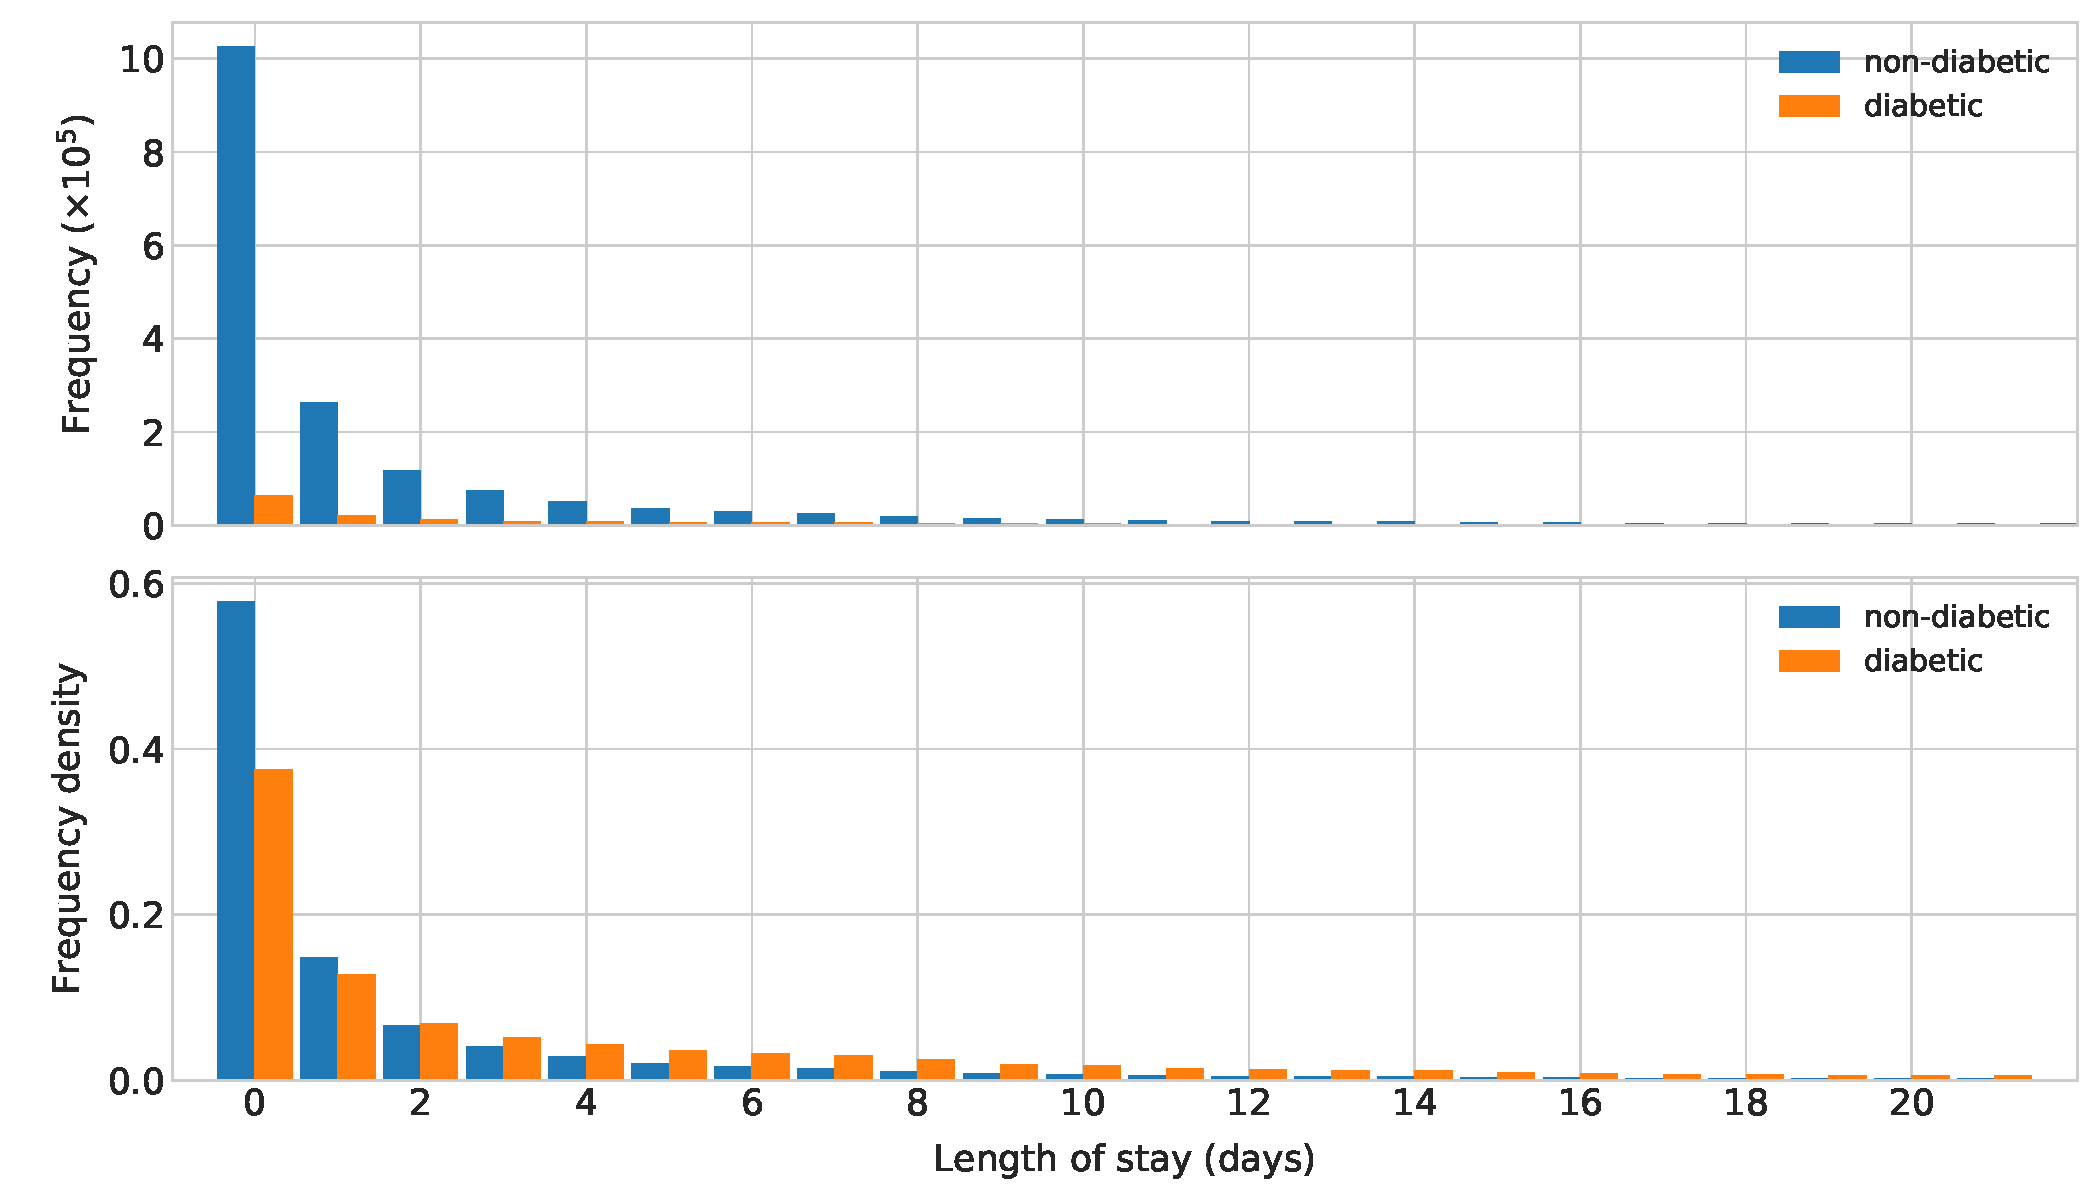
\includegraphics[width=\linewidth]{los_bar.pdf}
        }
    \end{minipage}\hfill%
    \begin{minipage}{.3\linewidth}
        \centering
        \textbf{\tiny{Length of stay}}
        \resizebox{\linewidth}{!}{%
            \begin{tabular}{lll}
\toprule
{} & Non-diabetic & Diabetic \\
\midrule
mean &         2.57 &     6.07 \\
std  &         8.13 &    12.55 \\
min  &         0.00 &     0.00 \\
1\%   &         0.00 &     0.00 \\
25\%  &         0.00 &     0.00 \\
50\%  &         0.00 &     1.00 \\
75\%  &         2.00 &     7.00 \\
99\%  &        35.00 &    57.00 \\
max  &       690.00 &   705.00 \\
\bottomrule
\end{tabular}

        }
    \end{minipage}\hfill%

    \begin{minipage}{.6\linewidth}
        \makebox[\linewidth]{%
            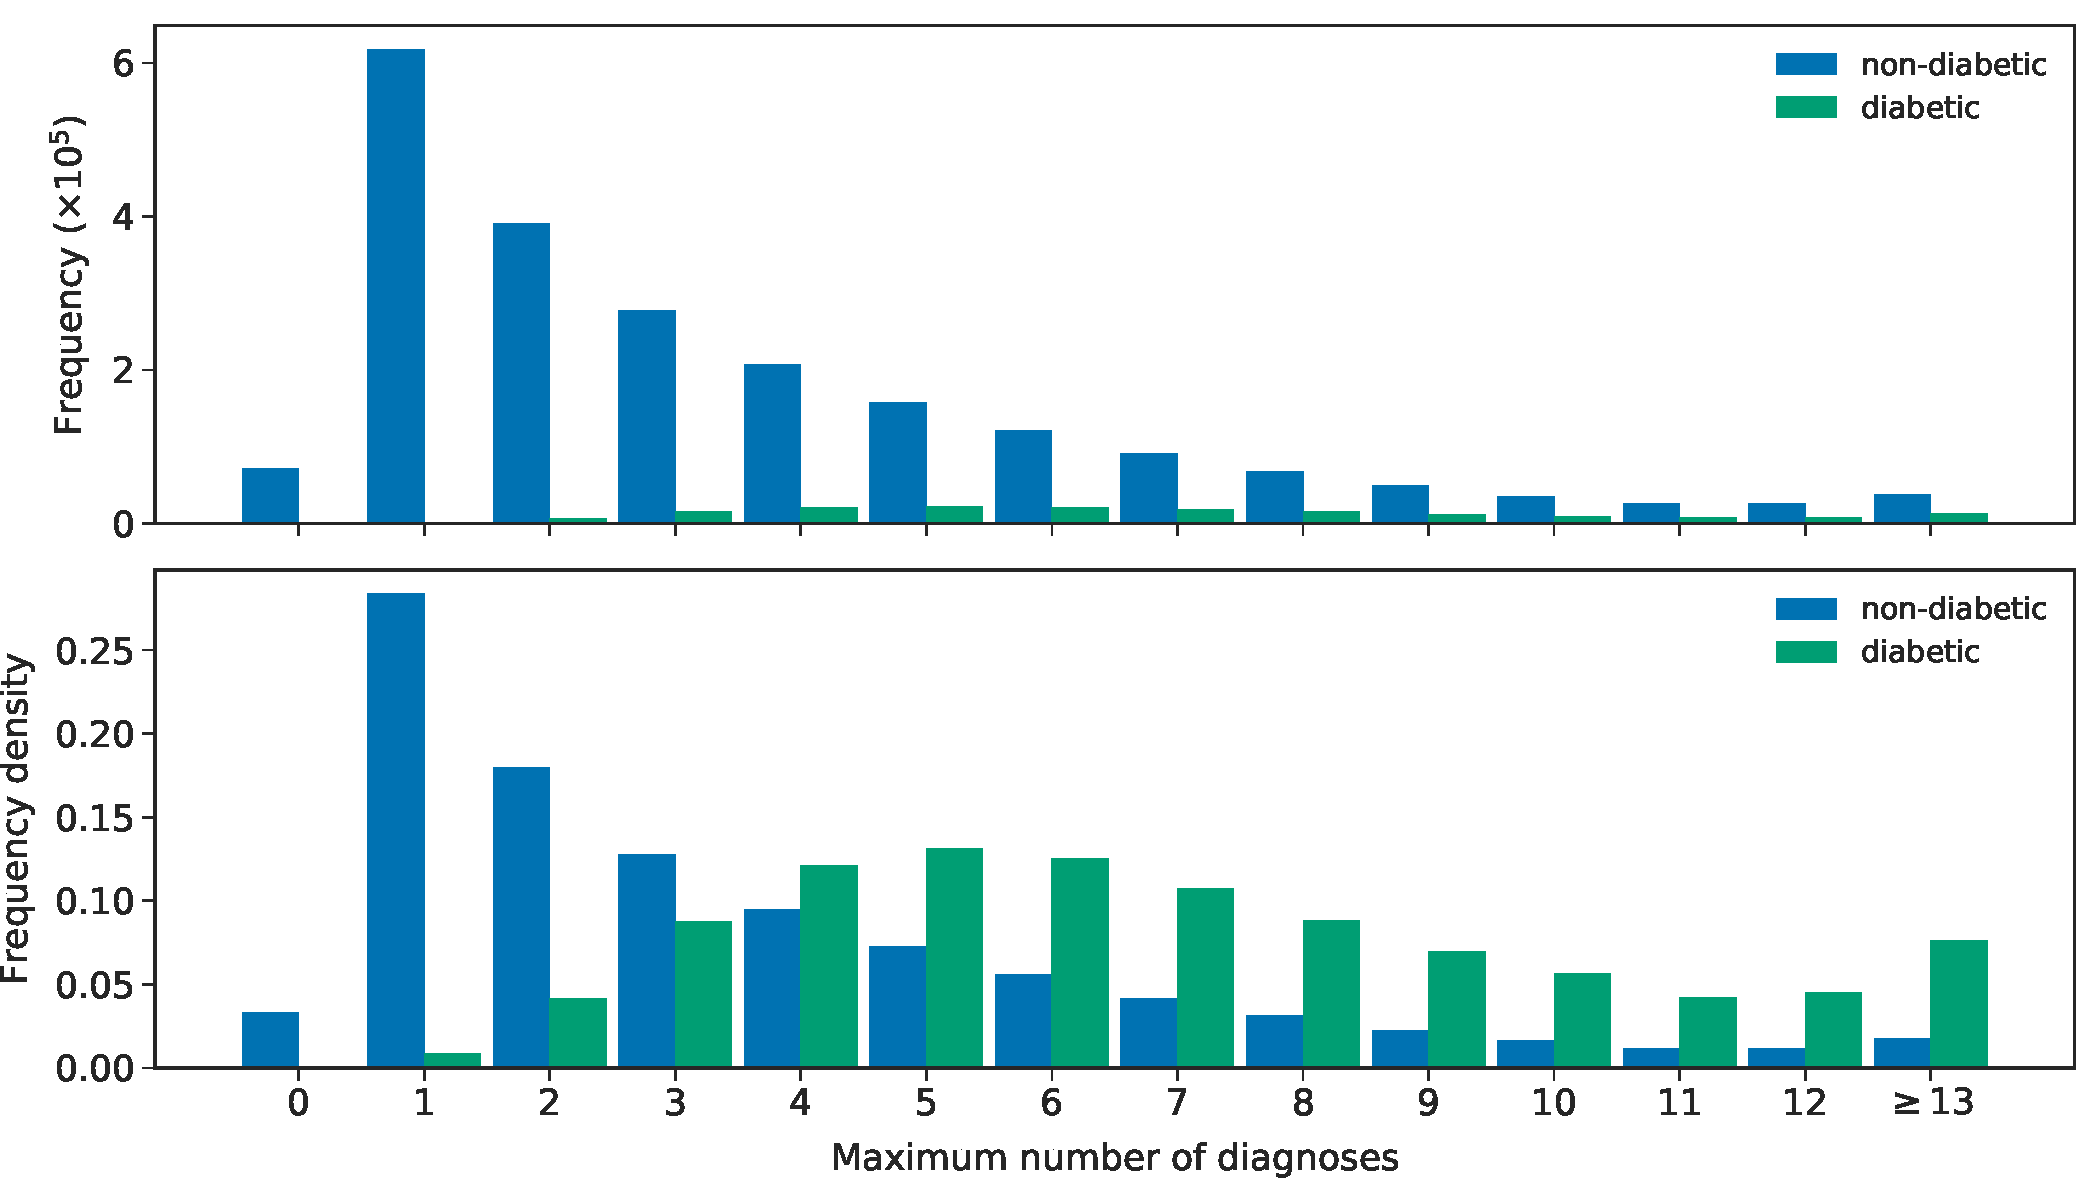
\includegraphics[width=\linewidth]{ndiag_bar.pdf}
        }
    \end{minipage}\hfill%
    \begin{minipage}{.3\linewidth}
        \centering
        \textbf{\tiny{Max.\ number of diagnoses}}
        \resizebox{\linewidth}{!}{%
            \begin{tabular}{lll}
\toprule
{} & Non-diabetic & Diabetic \\
\midrule
mean &         2.57 &     6.07 \\
std  &         8.13 &    12.55 \\
min  &         0.00 &     0.00 \\
1\%   &         0.00 &     0.00 \\
25\%  &         0.00 &     0.00 \\
50\%  &         0.00 &     1.00 \\
75\%  &         2.00 &     7.00 \\
99\%  &        35.00 &    57.00 \\
max  &       690.00 &   705.00 \\
\bottomrule
\end{tabular}

        }
    \end{minipage}\hfill%
}

%\frame{\frametitle{Net costs}
%    \makebox[\linewidth]{%
%        \begin{minipage}{.7\linewidth}
%            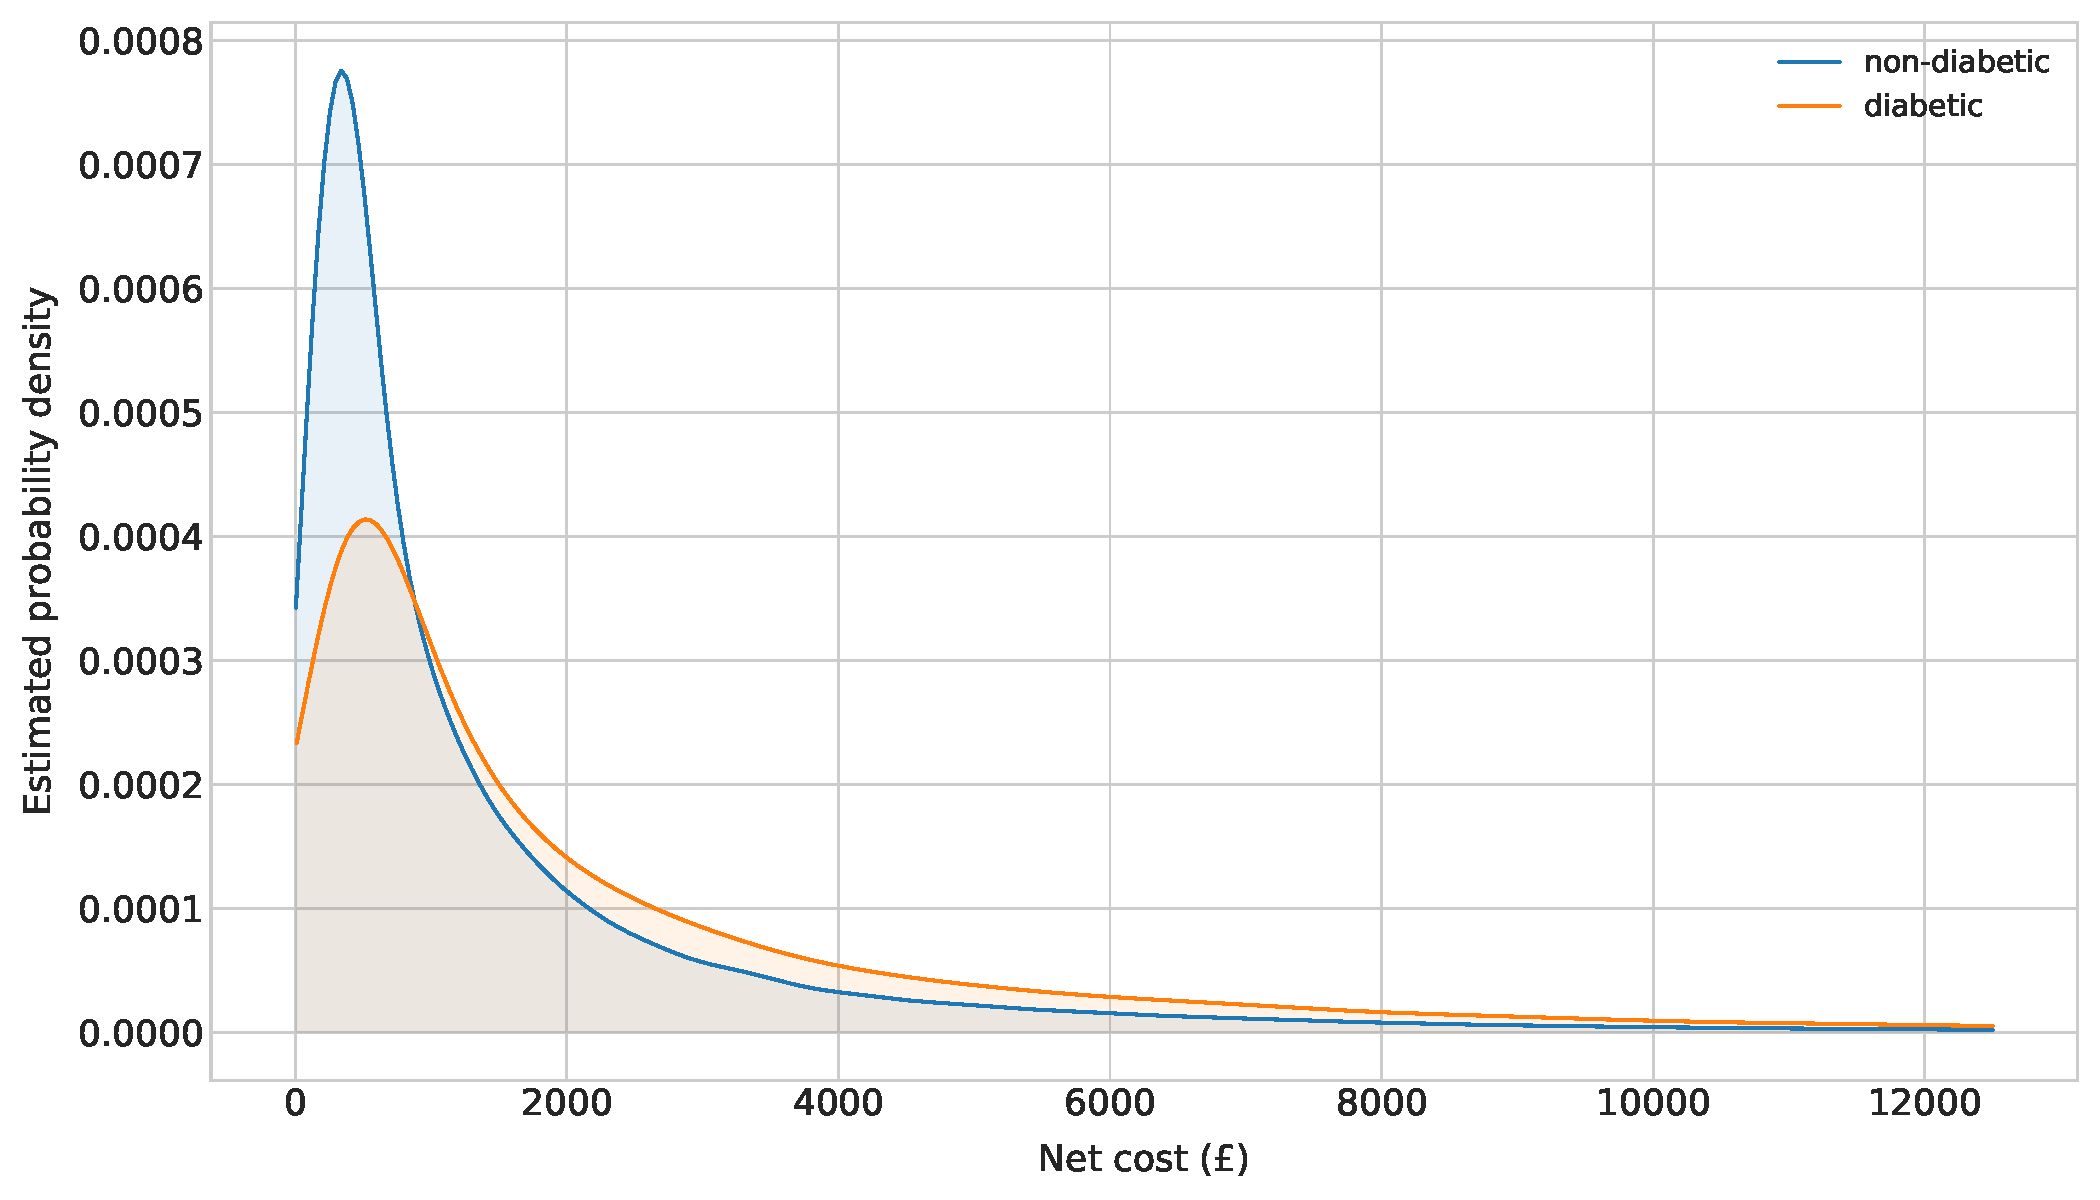
\includegraphics[width=\linewidth]{netcost_kde.pdf}
%        \end{minipage}\hfill%
%        \begin{minipage}{.25\linewidth}
%            \centering
%            \textbf{\tiny{Net cost of spell}}
%            \resizebox{\linewidth}{!}{%
%                \begin{tabular}{lll}
\toprule
{} & Non-diabetic &    Diabetic \\
\midrule
mean &     1,647.01 &    2,648.98 \\
std  &     3,019.54 &    4,152.20 \\
min  &         4.50 &       10.91 \\
1\%   &        62.55 &      139.65 \\
25\%  &       338.67 &      490.64 \\
50\%  &       709.33 &    1,227.95 \\
75\%  &     1,756.90 &    3,106.44 \\
95\%  &     6,179.92 &    9,591.06 \\
99\%  &    13,414.47 &   19,128.45 \\
max  &   369,168.93 &  273,450.30 \\
\bottomrule
\end{tabular}

%            }
%        \end{minipage}\hfill%
%    }
%}

\frame{\frametitle{Variation and importance}
    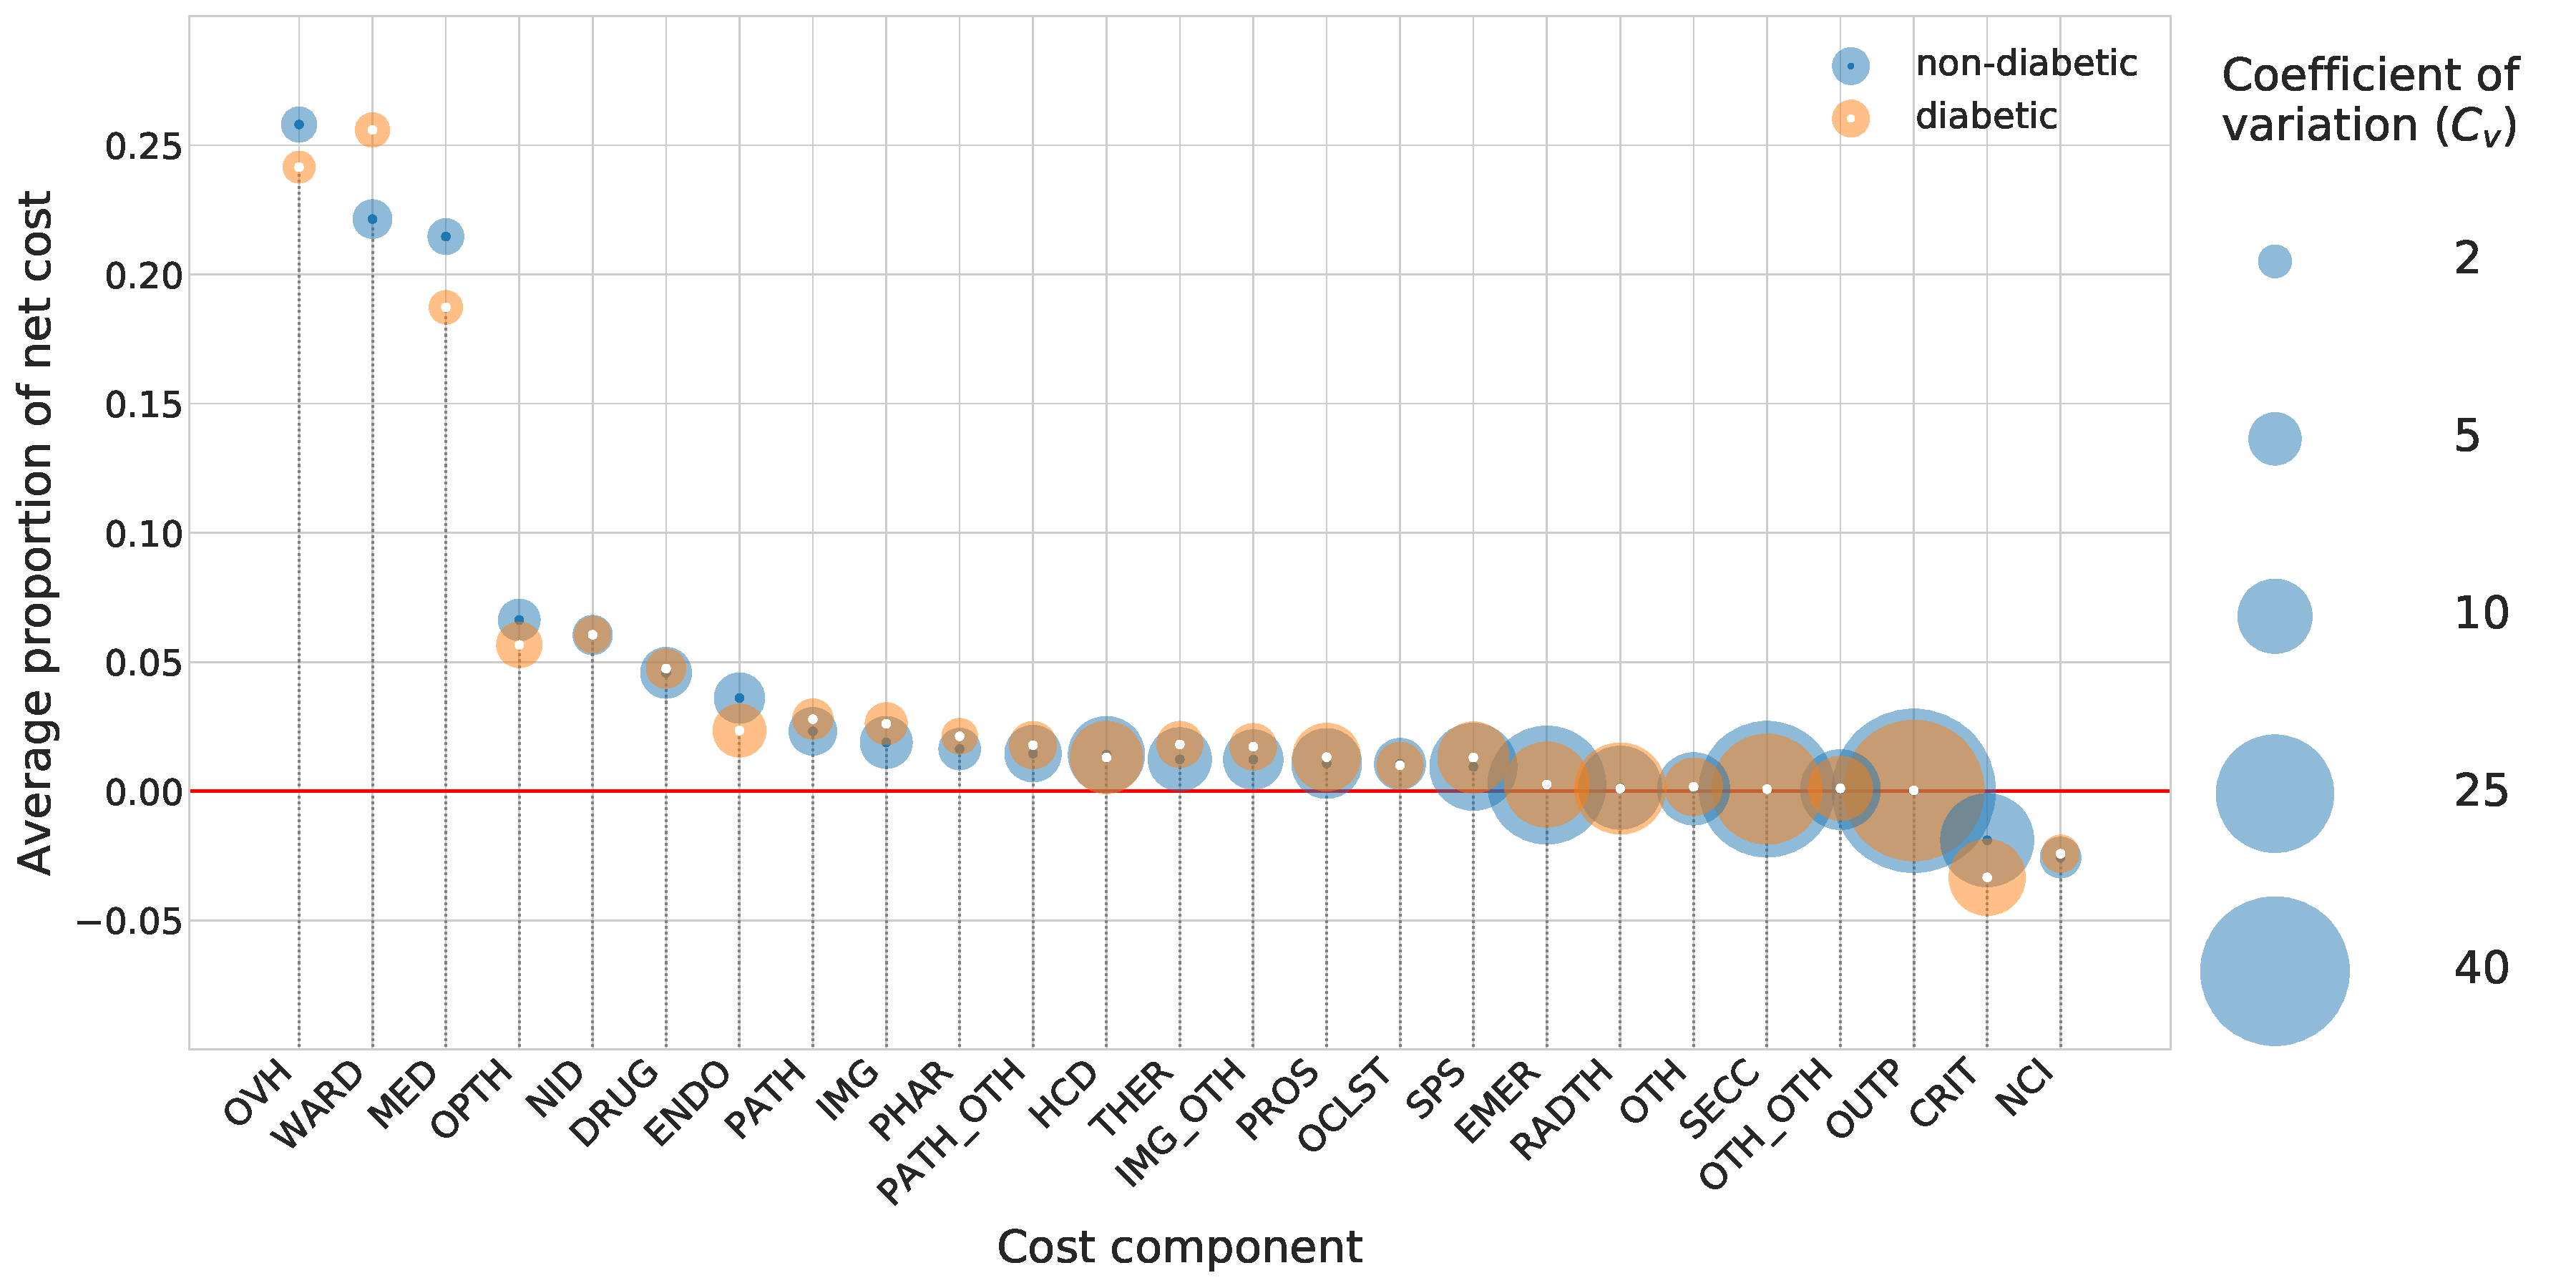
\includegraphics[width=\linewidth]{cost_bubble.pdf}
}


\section{Partitioning the data}

\frame{\frametitle{Subsets in the data}
    Traditional methods include~\footfullcite{Nolte2003}:

    \begin{itemize}
        \item condition-specific populations
        \item segmenting by age
    \end{itemize}

    However, these methods have the common flaw of under-representing groups of
    healthcare users~\footfullcite{Vuik2016}.
}

\frame{\frametitle{Misrepresentation \-- age}
    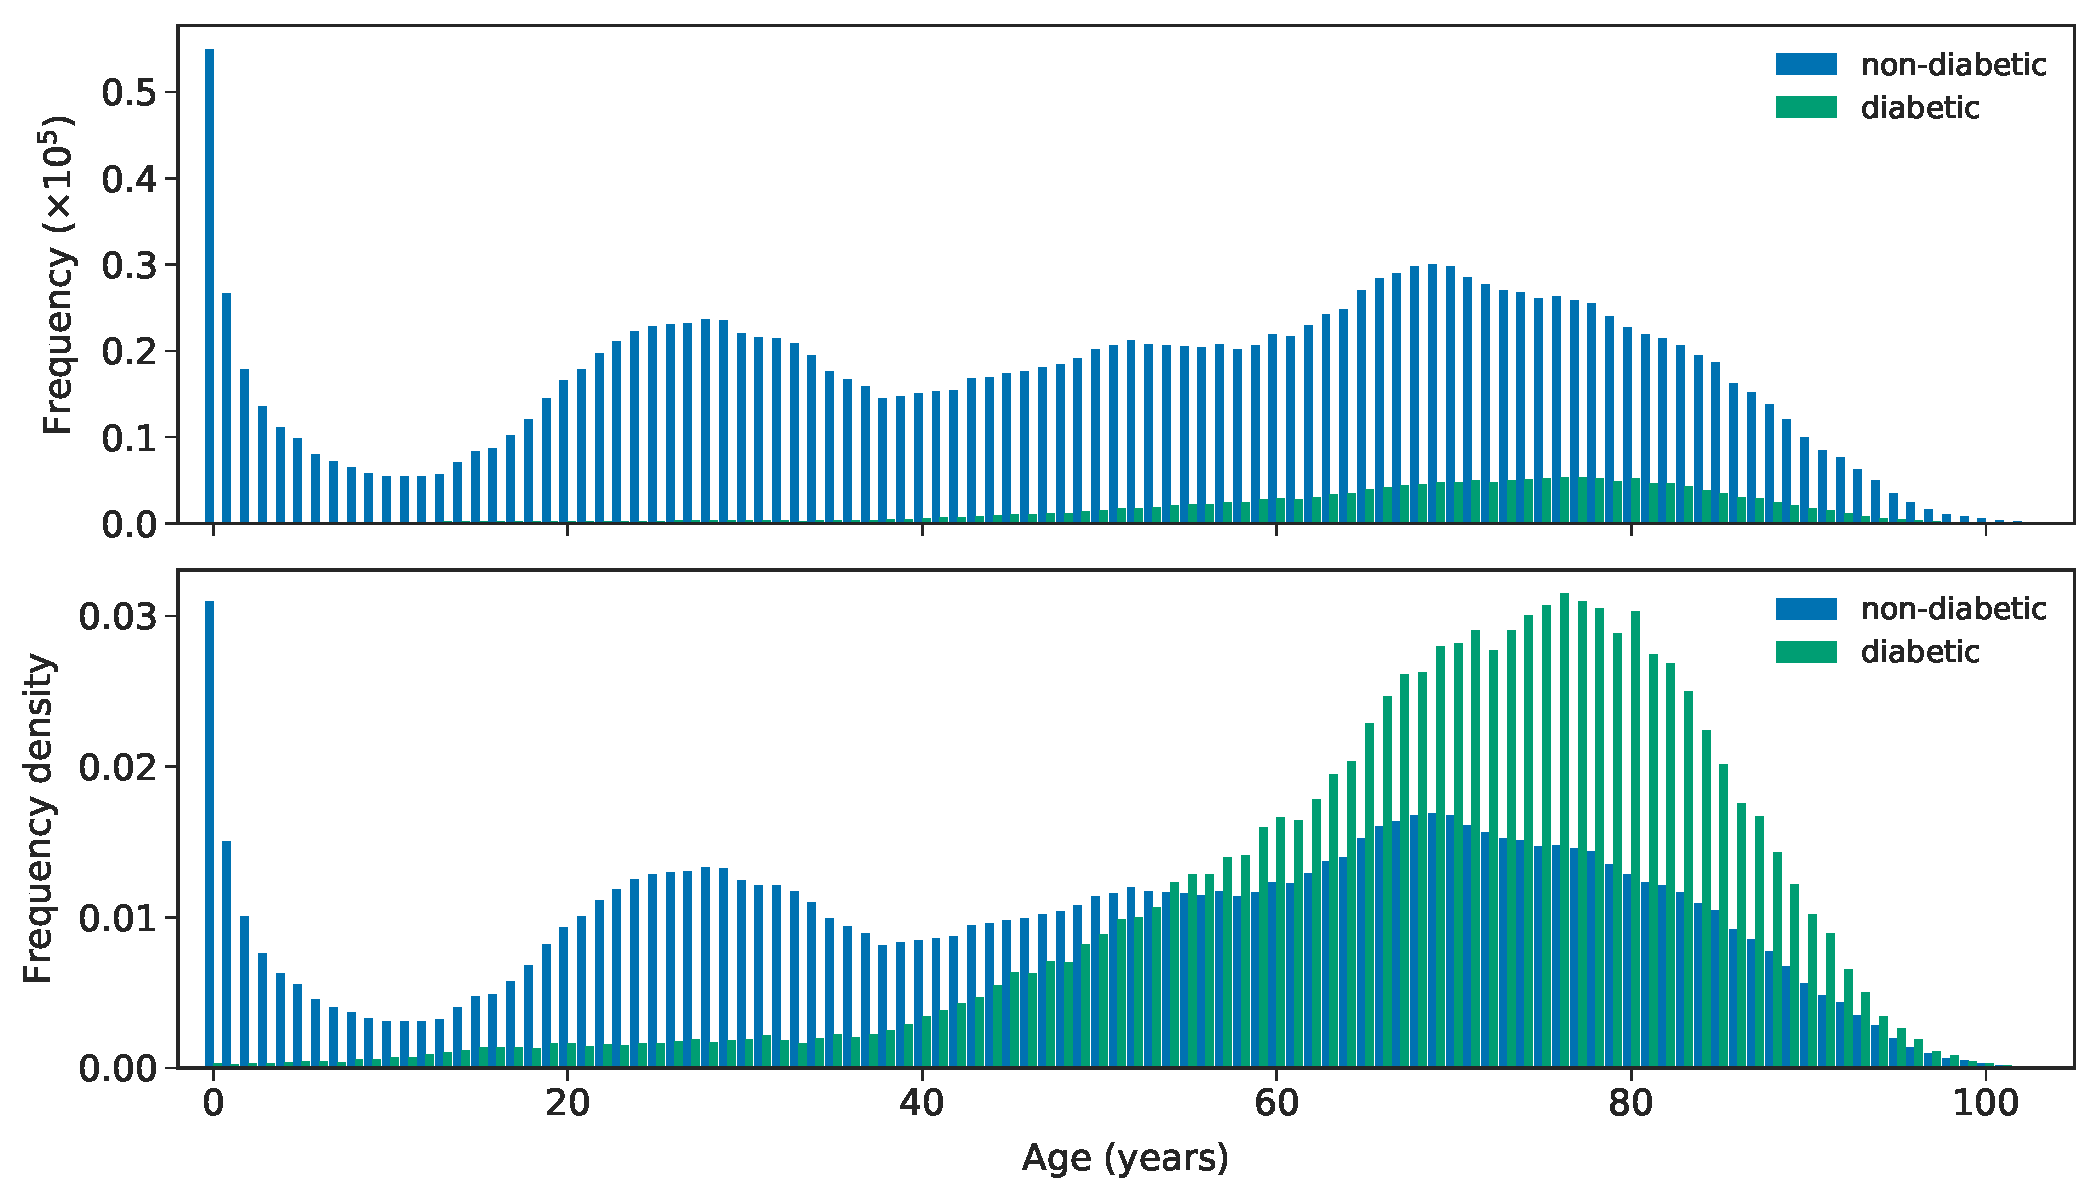
\includegraphics[width=\linewidth]{age_bar.pdf}
}

\frame{\frametitle{Misrepresentation \-- net cost of spell}
    \resizebox{\textwidth}{!}{%
        \begin{tabular}{llllll}
\toprule
{} & Non-diabetic &    Diabetic & Diabetic under 30 & Diabetic 30 to 65 & Diabetic 65 and over \\
\midrule
mean &     1,647.00 &    2,648.98 &          1,335.11 &          2,110.79 &             2,940.21 \\
std  &     3,019.53 &    4,152.20 &          2,034.58 &          3,565.45 &             4,415.44 \\
min  &         4.50 &       10.91 &             52.48 &             35.93 &                10.91 \\
1\%   &        62.55 &      139.65 &            125.54 &            129.63 &               143.83 \\
25\%  &       338.67 &      490.64 &            431.76 &            404.30 &               546.11 \\
50\%  &       709.32 &    1,227.95 &            840.28 &            990.53 &             1,395.78 \\
75\%  &     1,756.90 &    3,106.44 &          1,605.21 &          2,338.76 &             3,584.18 \\
95\%  &     6,179.79 &    9,591.06 &          3,698.95 &          7,551.34 &            10,457.59 \\
99\%  &    13,414.48 &   19,128.45 &          7,697.49 &         16,277.28 &            20,310.51 \\
max  &   369,168.93 &  273,450.30 &         66,963.80 &        106,860.69 &           273,450.30 \\
\bottomrule
\end{tabular}

    }
}

\graphicspath{{img/clustering/}}
\frame{\frametitle{What is clustering?}
    \begin{figure}[htbp]
        \centering
        \animategraphics[loop,
                         controls,
                         width=.5\imgwidth]{1}{kmeans-}{0}{12}
    \end{figure}

    \footnotesize Image taken from \url{%
        https://www.jeremyjordan.me/
        grouping-data-points-with-k-means-clustering/
    }
}

\frame{\frametitle{Clustering with healthcare data}

    \begin{itemize}
        \item Patient pathways
            \begin{itemize}
                \item[] \fullcite{Rebuge2012}
            \end{itemize}
        \item Utilisation patterns
            \begin{itemize}
                \item[] \fullcite{Vuik2016}
            \end{itemize}
    \end{itemize}
}



\frame{\frametitle{Take home message}
    \Large
    \begin{itemize}
        \item Don't impose a framework
        \item Data-driven solutions
        \item Let the data speak for itself
    \end{itemize}
}

\end{document}
